\documentclass[11pt]{article}

\usepackage[a4paper,margin=2.0cm]{geometry}
\usepackage{booktabs}
\usepackage{amsmath}
\usepackage{siunitx}
\usepackage[hidelinks]{hyperref}
\usepackage{parskip}
\usepackage{titlesec}
\usepackage{graphicx}
\usepackage{subcaption}
\graphicspath{{data/}}

\titlespacing*{\section}{0pt}{1.1ex plus .3ex}{0.5ex}
\titlespacing*{\subsection}{0pt}{0.8ex plus .2ex}{0.3ex}
\titleformat{\section}{\normalfont\large\bfseries}{\thesection}{0.6em}{}
\setlength{\parskip}{0.5ex}

\title{\vspace{-1.2cm}\textbf{Population Growth and CO\textsubscript{2} Emissions:\\ A Worldwide Analysis}}
\author{Data-analysis report prepared in R (tidyverse)}
\date{\today}
\vspace{-1.5cm}

\begin{document}
\maketitle

\begin{abstract}
\noindent
This study examines whether the size of a country's population is related to its
carbon dioxide (CO\textsubscript{2}) emissions, using the Kaggle \emph{World
Population Dataset} (234 countries and territories, 17 variables) and the
\emph{CO2 Emission Around the World} dataset (per-capita emissions, 1990--2019).
The data were managed and analysed entirely in R with the tidyverse. After
cleaning---standardising column names, removing duplicates, imputing missing
values with the median, and winsorising rate variables by the inter-quartile
range---an exploratory analysis described the structure and quality of the
population data. A new variable, each country's projected 2030 population, was
created with the exponential growth model $N_t = P e^{rt}$; the world total is
projected to rise from 7.97 billion in 2022 to 8.57 billion in 2030
($+7.5\%$). The ten most populous countries and their 1990--2022 population and
1990--2019 emission trends were visualised with ggplot2. Correlation and linear
regression were then used on 172 countries matched across both datasets. The
association between 2022 population and 2019 per-capita emissions was found to be
negligible (Pearson $r = 0.015$; regression slope $-0.171$, $p = 0.67$,
$R^2 \approx 0.001$): population size does not predict per-capita emissions.
Summing 2019 per-capita emissions by continent placed Asia first and South
America last. The main lesson is that emission intensity is driven by economic
and energy structure, not by headcount, which has direct implications for how
climate responsibility is interpreted.
\end{abstract}

\section{Introduction}
Population growth is often cited as a driver of rising greenhouse-gas emissions.
Yet emissions depend not only on \emph{how many} people live in a country but on
\emph{how} they produce and consume energy. This report tests the population
--emissions link empirically. The objectives follow the assignment brief:
(i) manage and clean the population data; (ii) perform exploratory data analysis
(EDA); (iii) engineer a projected-population variable; (iv) visualise population
and emission trends for the largest countries; (v) quantify correlations,
including a merged population--emissions analysis; and (vi) compare emissions
across continents.

\section{Methods}
\subsection{Datasets}
The \textbf{World Population Dataset} contains 234 rows and 17 columns: rank,
country code (CCA3), country/territory, capital, continent, population snapshots
for 1970, 1980, 1990, 2000, 2010, 2015, 2020 and 2022, land area
(km\textsuperscript{2}), density, growth rate and world-population percentage.
The \textbf{CO2 Emission Around the World} dataset gives annual CO\textsubscript{2}
emissions in metric tons per capita for each country from 1990 to 2019 (the file
shipped a duplicated 2019 column, which was de-duplicated during loading).

\subsection{Tools and procedure}
All work was done in R~4.6 using the tidyverse (\texttt{readr}, \texttt{dplyr},
\texttt{tidyr}, \texttt{ggplot2}) with \texttt{janitor}, \texttt{scales} and
\texttt{corrplot}, and knitted to HTML with \texttt{rmarkdown}/\texttt{knitr}.
Cleaning used \texttt{clean\_names()} for consistent naming,
\texttt{distinct()} for duplicate removal, median imputation for missing numeric
values, and IQR winsorising for the rate variables (density, growth rate,
world-population percentage) used in the correlation study; genuine large-country
values in the population columns were retained. Box plots were used to inspect
outliers. The 2030 projection used the exponential model
\[
N_t = P\,e^{rt},\qquad P = \text{2022 population},\; t = 8,\;
r = (\text{growth-rate factor}) - 1 .
\]
The two datasets were merged on country name (after normalising well-known name
differences such as ``Russian Federation'' $\rightarrow$ ``Russia''), retaining
2022 population and 2019 emissions for 172 matched countries.

\section{Results}
\subsection{EDA and projection (Tasks 4.2--4.3)}
The population data were complete after cleaning, with no duplicate rows.
Population columns are strongly right-skewed---China and India are genuine
extremes rather than errors. Applying the growth model, the world population is
projected to grow from \num{7973413042} (2022) to \num{8569157744} (2030). Growth
is highly uneven: Nigeria is projected to grow by about 21\%, while China, whose
growth rate is effectively zero, stays flat and is overtaken in momentum by India
(Table~\ref{tab:top10}).

\begin{table}[h]
\centering
\caption{Ten most populous countries: 2022 population and projected 2030 population.}
\label{tab:top10}
\small
\begin{tabular}{llrr}
\toprule
Country & Continent & 2022 population & Projected 2030 \\
\midrule
China          & Asia          & \num{1425887337} & \num{1425887337} \\
India          & Asia          & \num{1417173173} & \num{1496402904} \\
United States  & North America & \num{338289857}  & \num{348731782}  \\
Indonesia      & Asia          & \num{275501339}  & \num{289974355}  \\
Pakistan       & Asia          & \num{235824862}  & \num{274757645}  \\
Nigeria        & Africa        & \num{218541212}  & \num{265011868}  \\
Brazil         & South America & \num{215313498}  & \num{223384633}  \\
Bangladesh     & Asia          & \num{171186372}  & \num{186634630}  \\
Russia         & Europe        & \num{144713314}  & \num{141621023}  \\
Mexico         & North America & \num{127504125}  & \num{134095029}  \\
\bottomrule
\end{tabular}
\end{table}

\subsection{Trends for the largest countries (Task 4.4)}
Bar and line charts (see the accompanying \texttt{analysis.html}) show that the
populations of the ten largest countries rose steadily from 1990 to 2022, led by
China and India. Their per-capita emission trends (1990--2019) diverge sharply:
the United States has high but gradually declining per-capita emissions, China's
rose steeply before levelling, while India, Nigeria and Bangladesh remain low per
capita despite very large populations.

\subsection{Trends for the largest countries (Task 4.4)}
Figure~\ref{fig:trends} shows that the populations of the ten largest countries
rose steadily from 1990 to 2022, led by China and India. ...

\begin{figure}[htbp]
  \centering
  \begin{subfigure}[b]{0.49\textwidth}
    \centering
    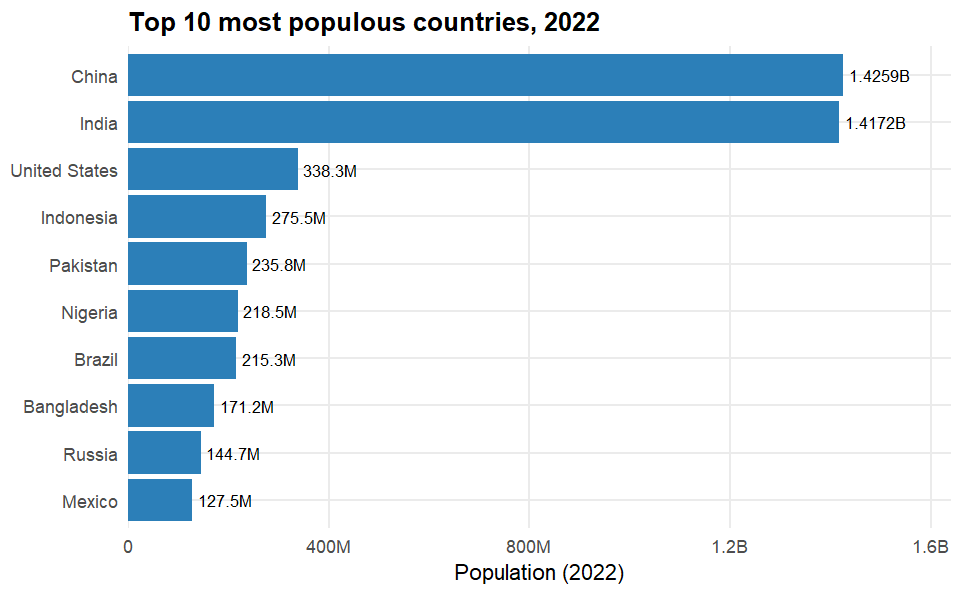
\includegraphics[width=\textwidth]{largest_countries.png}
    \caption{Population, 1990--2022}
    \label{fig:pop_trend}
  \end{subfigure}
  \hfill
  \begin{subfigure}[b]{0.49\textwidth}
    \centering
    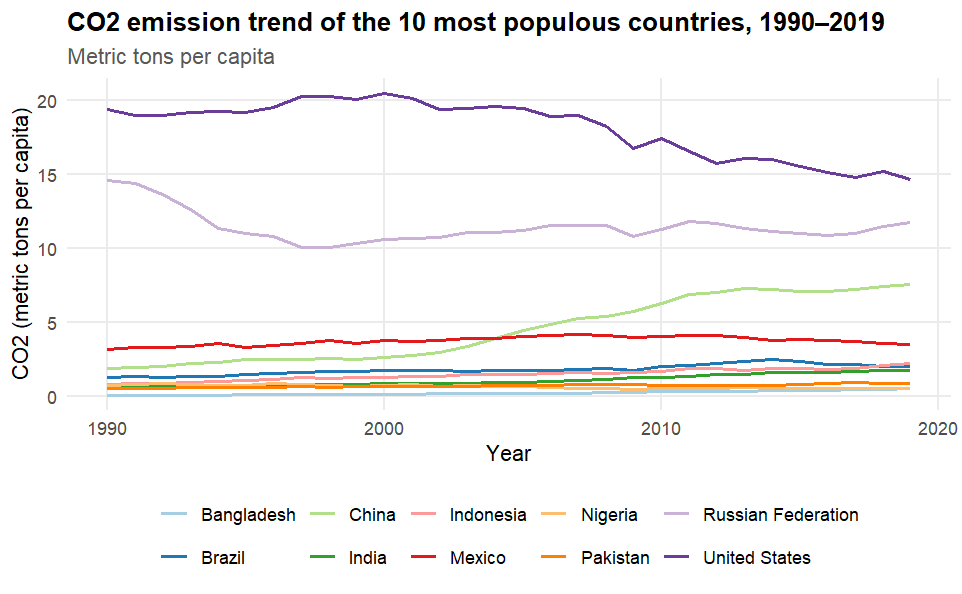
\includegraphics[width=\textwidth]{co2_emission.png}
    \caption{CO\textsubscript{2} per capita, 1990--2019}
    \label{fig:co2_trend}
  \end{subfigure}
  \caption{Population and per-capita emission trends for the ten most populous countries.}
  \label{fig:trends}
\end{figure}

\subsection{Correlation and regression (Task 4.5)}
Among the population variables, pairwise correlations between area, density,
growth rate and world-population percentage are weak, the clearest being a
positive link between land area and world-population share. For the merged data,
the relationship between 2022 population and 2019 per-capita emissions is
\emph{negligible}: Pearson $r = 0.015$, Spearman $\rho = -0.088$, and a linear
regression of per-capita emissions on $\log_{10}(\text{population})$ gives a slope
of $-0.171$ ($p = 0.67$) with $R^2 \approx 0.001$. Population size therefore
explains virtually none of the variation in per-capita emissions.

\subsection{Continental comparison (Task 4.6)}
Table~\ref{tab:cont} sums 2019 per-capita emissions by continent.
\textbf{(1)} The highest-emitting continent is \textbf{Asia}
(\num{261.42} metric tons per capita summed). \textbf{(2)} The third continent is
\textbf{North America}, totalling \num{79.57} metric tons per capita.
\textbf{(3)} The lowest is \textbf{South America}, at \num{29.42} metric tons per
capita. Because this is a \emph{sum} of per-capita values, the totals are
influenced by how many countries each continent contributes; on a per-country
mean basis Asia (6.70) and Europe (5.88) remain highest and Africa lowest (1.23).

\begin{table}[h]
\centering
\caption{Total and mean 2019 CO\textsubscript{2} (metric tons per capita) by continent, matched countries.}
\label{tab:cont}
\small
\begin{tabular}{lrrr}
\toprule
Continent & Total & Mean & Countries \\
\midrule
Asia          & 261.42 & 6.70 & 39 \\
Europe        & 240.97 & 5.88 & 41 \\
North America & 79.57  & 4.19 & 19 \\
Africa        & 60.50  & 1.23 & 49 \\
Oceania       & 53.20  & 4.09 & 13 \\
South America & 29.42  & 2.67 & 11 \\
\bottomrule
\end{tabular}
\end{table}

\section{Discussion}
The headline result is that a country's population size is essentially unrelated
to its per-capita CO\textsubscript{2} emissions. This is consistent with climate
science: per-capita emissions reflect income levels, energy mix and industrial
structure rather than headcount. Highly populous but lower-income countries
(India, Nigeria, Bangladesh) have low per-capita emissions, whereas smaller,
energy-intensive economies emit far more per person. The continental comparison
must be read with care, because summing a per-capita rate rewards continents with
many countries; the per-country means give a fairer ranking and still show Asia
and Europe ahead of Africa.

\section{Lessons learned and recommendations}
The project reinforced several practical points. First, \emph{data quality work
dominates}: the duplicated 2019 column silently emptied the merge until it was
handled, showing why loading should always be validated. Second, \emph{units
matter}---summing a per-capita metric answers the literal question but can
mislead; totals and means should be reported together. Third, \emph{robust code}
(auto-detecting files, matching year columns by pattern, normalising country
names) makes an analysis reproducible. Recommendations: (i) analyse
\emph{total} (not only per-capita) emissions to assess absolute climate impact;
(ii) bring in GDP and energy-mix variables, which should explain emissions far
better than population; and (iii) reconcile country naming with ISO codes before
merging to avoid losing records.

\section{Conclusion}
Using the tidyverse, this study cleaned and projected world population data,
visualised trends for the largest countries, and tested the population--emissions
link. Population is projected to reach 8.57 billion by 2030, but its size shows no
meaningful correlation with per-capita emissions ($R^2 \approx 0.001$). Emission
intensity is a function of how economies are powered, not of how many people they
hold---an important distinction for interpreting national climate responsibility.

\end{document}
